% \todo{ Double Check the checklist}
\appendix
\onecolumn
\section{Experimental Setup}
\subsection{Model Details}
\label{app:model_details}
\textbf{Model:}
For most of our MiniHack experiments, we use a 100M causal transformer model with \texttt{num\_layers = 12}, \texttt{d\_model = 768}, and \texttt{num\_heads = 12}. For our model scaling experiments presented in \Cref{sec:dataset_size}, we consider the following values for \texttt{num\_layers}, \texttt{d\_model}, and \texttt{num\_heads} presented in \Cref{tab:model_details}. For procgen experiments, we use a 210M causal transformer with \texttt{num\_layer = 12} , \texttt{d\_model = 1024} and \texttt{n\_heads = 16}. 

\begin{table}[h!]
\centering
\begin{tabular}{c c c c}
\hline
Number of Parameters & \texttt{num\_layers} & \texttt{d\_model} & \texttt{num\_heads} \\
\hline\hline
1M & 4 & 128 & 4\\
10M & 6 & 256 & 8 \\
30M & 8 & 512 & 8 \\
100M & 12 & 768 & 12 \\
200M & 12 & 1024 & 16 \\
310M & 18 & 1024 & 16 \\
\hline
\end{tabular}

\caption{List of transformer model configurations with varying number of parameters, including details on the number of layers, model dimension, and the number of attention heads.}

\label{tab:model_details}
\end{table}

For embedding the minihack observations, we use the \texttt{NetHackStateEmbeddingNet} from \href{https://github.com/facebookresearch/e3b/blob/main/minihack/src/models.py#L589}{https://github.com/facebookresearch/e3b/blob/main/minihack/src/models.py}. For embedding actions and rewards, we follow the same procedure as \cite{decision_transformer}. For the experiments presented in \Cref{sec:analysis}, we stack $3$ episodes along the sequence axis and restrict the context size to $900$ tokens. Since the episodes are of variable length, we stack the three episodes contiguously and then pad the rest of the sequence with padding tokens. For the MiniHack main results presented in \Cref{sec:main_results}, we stack $8$ episodes from the same level (i.e., $p_b = 1.0$) and use the context length of $2048$. Similarly for Procgen results presented in the same section, we stack $4$ episodes from the same level and use the context length of $2048$.

\textbf{Training:} For all our experiments, we use AdamW optimizer \citep{shen2023unified} for optimization with cosine annealing learning rate scheduler. We train our models for 25 epochs in case of MiniHack and 100 epochs for Procgen environments. 

\subsubsection{Compute} We use 8 GPUs, each with 80GB of RAM, leveraging PyTorch's Distributed Data Parallel (DDP) capabilities for training. The largest model in our MiniHack experiments (100M), trained on a dataset comprising 100K MiniHack levels with a batch size of 64, took approximately 42 hours (1 day and 18 hours) for complete training. We emphasize that it is feasible to conduct the training with a single GPU; however, this approach would extend the training duration. For inference tasks, we utilize 1 GPU.


\subsection{Environment Details}
\label{app:env_details}
\subsubsection{MiniHack}
\textbf{Observation Space - }
The observation space in MiniHack is designed as a dictionary-style structure. It primarily borrows keys from the foundational NetHack Learning Environment (NLE), with the addition of a few unique keys specific to MiniHack. To get the necessary observations from the environment, relevant options need to be specified during the initialization process. In this paper, we focus on a few key observation types:
\begin{enumerate}
    \item \textbf{Glyphs}: This refers to a 21x79 matrix comprising glyphs, which are identifiers of entities present on the map. Each glyph is unique and represents a specific entity. They are represented as integers ranging from 0 to 5991.
    \item \textbf{Blstats}: This is a 26-dimensional vector that displays the status line found at the screen's bottom. It provides information about the player character's location, health status, attributes, and other vital statuses.
    \item \textbf{Messages}: This is a 256-dimensional vector that represents the UTF-8 encoding of the message displayed on the screen's top. 
\end{enumerate}


\textbf{Action Space - } In this work, all of our environments are navigation-based, and therefore, the action space consists of eight compass directions. Additionally, we create a padding action represented by the number 31 for padding purposes.

\textbf{Rewards - } In all MiniHack environments, the rewards are sparse. In other words, the agent receives a reward of +1 if it successfully solves the task at hand, and 0 otherwise. The environment also penalizes the agent for bumping into lava, monsters, or walls. 

In our work, we consider the following environments - 
\begin{enumerate}
    \item \texttt{MiniHack-MultiRoom-N6-v0} -  In this task, the agent must navigate through six rooms and reach the goal. Upon reaching the goal, the agent receives a reward of $+1$, otherwise, the reward is $0$. Collisions with walls incur a penalty of $-0.01$.
    \item \texttt{MiniHack-MultiRoom-N6-Lava-v0} - In this task, the agent navigates through six rooms with lava-covered walls. The task is completed with a reward of $+1$ when the goal is reached; otherwise, the reward is $0$. Collisions with lava result in immediate death.
    \item \texttt{MiniHack-MultiRoom-N4-Lava-v0} - This task is similar to \texttt{MiniHack-MultiRoom-N6-Lava-v0}, but with only four rooms. The agent must avoid lava-filled walls to complete the task.The task is completed with a reward of $+1$ when the goal is reached; otherwise, the reward is $0$. Collisions with lava result in immediate death.
    \item \texttt{MiniHack-MazeWalk-9x9-v0} - The agent navigates a $9 \times 9$ maze. Upon reaching the goal, the agent receives a reward of $+1$ otherwise, the reward is $0$. Collisions with walls incur a penalty of $-0.01$. 
    \item \texttt{MiniHack-CorridorBattle-Dark-v0} -  The agent must battle the monsters strategically in a dark room, using corridors for isolation. The agent must keep track of its kill count. A reward of $+1$ is given upon survival, otherwise the agent receives a reward of $0$. 
    \item \texttt{MiniHack-MultiRoom-N6-LavaMonsters-v0} - The agent must navigate through six rooms filled with monsters and lava. To successfully complete this task, the agent must avoid the lava walls and monsters.  The agent receives a reward of $+1$, otherwise $0$. 
    \item \texttt{MiniHack-MultiRoom-N6-Open-v0} - The agent navigates through six rooms without doors. The reward structure is identical to that of \texttt{MiniHack-MultiRoom-N6-v0}.
    \item \texttt{MiniHack-MultiRoom-N10-LavaOpen-v0} - In this task, the agent navigates through ten rooms to reach the goal. Collisions with lava walls result in immediate death. Upon reaching the goal, the agent receives a reward of $+1$.
    \item \texttt{MiniHack-SimpleCrossingS11N5-v0} -  Here, the agent reaches the goal on the other side of the room. The agent receives a reward of $+1$ for reaching the goal, a penalty of $-0.01$ for hitting the walls, and $0$ otherwise.
    \item \texttt{MiniHack-SimpleCrossingS9N2-v0} - This task is an easier version of \texttt{MiniHack-SimpleCrossingS11N5-v0}.
    \item \texttt{MiniHack-River-Narrow-v0} - The agent crosses a river by using boulders to create a dry path, aiming to reach the goal on the other side. The agent receives a reward of $+1$ upon reaching the goal.
    \item \texttt{MiniHack-HideNSeek-v0} - The agent is placed in a room filled with sight-blocking trees and clouds. The agent must avoid monsters while navigating the environment to reach the goal swiftly.
    \item \texttt{MiniHack-MultiRoom-N2-Monster-v0} -  The agent must navigate through two rooms, avoiding monsters. It receives a reward of +1 upon reaching the goal and otherwise 0. 
    \item \texttt{MiniHack-LavaCrossingS11N5-v0} - This task is similar to SimpleCrossing, but the environment is filled with several lava streams running across the room, either horizontally or vertically. The agent needs to avoid the lava, as touching it would result in immediate death.
    The agent receives a reward of +1 upon the completion of the task. 
    \item \texttt{MiniHack-Memento-F2-v0} - In this task, the agent is presented with a cue at the beginning of the episode and the agent must navigate through the corridor. The end of corridor leads to a two-path fork and the agent should choose one direction based on the cue it saw in the beginning. Upon choosing the correct path and reaching the goal, the gent receives +1 reward and -1 for stepping on the trap. 
    \item \texttt{MiniHack-Memento-F4-v0} - In this task, the agent is presented with a cue at the beginning of the episode and the agent must navigate through the corridor. The end of corridor leads to a four-path fork and the agent should choose one direction based on the cue it saw in the beginning. Upon choosing the correct path and reaching the goal, the gent receives +1 reward and -1 for stepping on the trap. 
    \item \texttt{MiniHack-MazeWalk-15x15-v0} - This task is a slightly harder task than \texttt{MiniHack-MazeWalk-15x15-v0}. The agent navigates a $15 \times 25$ maze. Upon reaching the goal, the agent receives a reward of $+1$ otherwise, the reward is $0$. Collisions with walls incur a penalty of $-0.01$. 
    \item \texttt{MiniHack-MazeWalk-45x15-v0} - This task is a very challenging task than \texttt{MiniHack-MazeWalk-9x9-v0} The agent navigates a $45 \times 15$ maze. Upon reaching the goal, the agent receives a reward of $+1$ otherwise, the reward is $0$. Collisions with walls incur a penalty of $-0.01$. 
    \item \texttt{MiniHack-Labyrinth-Small-v0} - This task is a very challenging task than \texttt{MiniHack-MazeWalk-9x9-v0} The agent navigates a $45 \times 15$ maze. Upon reaching the goal, the agent receives a reward of $+1$ otherwise, the reward is $0$. Collisions with walls incur a penalty of $-0.01$. 
\end{enumerate}

For the task diversity experiments presented in \Cref{sec:dataset_size}, we use the environments in \Cref{tab:minihack_env_details}. Note that we randomly sample these environments to avoid selection bias. 


% 'simple_crossing_11_5', 'multiroom_10_lava_open', 'six_rooms', 'multiroom_4_lava', 'multiroom_6_lava', 'maze_walk_9', 'multiroom_6_lava_open', 'corridor_battle' 
% 'lava_crossing', 'multiroom_10_lava_open', 'river_narrow', 'six_rooms'
\begin{table}[!ht]
\centering
\begin{tabular}{c c }
\hline
\textbf{Number of Tasks} & \textbf{Environments} \\
\hline
1 Task  & \texttt{MiniHack-MultiRoom-N6-v0},  \\
\hline
4 Tasks & \texttt{MiniHack-LavaCrossingS11N5-v0} \\
        & \texttt{MiniHack-MultiRoom-N6-v0}\\
        & \texttt{MiniHack-River-Narrow-v0}\\
        & \texttt{MiniHack-MultiRoom-N10-LavaOpen-v0} \\
\hline

8 Tasks &  \texttt{MiniHack-SimpleCrossingS11N5-v0} \\
        & \texttt{MiniHack-MultiRoom-N10-LavaOpen-v0}\\
        &  \texttt{MiniHack-MultiRoom-N6-v0} \\
        & \texttt{MiniHack-MultiRoom-N6-Lava-v0} \\
        &  \texttt{MiniHack-MultiRoom-N4-Lava-v0} \\
        &  \texttt{MiniHack-MazeWalk-9x9-v0} \\
        &   \texttt{MiniHack-MultiRoom-N6-LavaOpen-v0} \\
        &\texttt{MiniHack-CorridorBattle-Dark-v0} \\
\hline

12 Tasks & \texttt{MiniHack-MultiRoom-N6-v0}\\
        & \texttt{MiniHack-MultiRoom-N6-Lava-v0} \\ 
        &  \texttt{MiniHack-MazeWalk-9x9-v0}\\
        &\texttt{MiniHack-CorridorBattle-Dark-v0}\\
        &  \texttt{MiniHack-MultiRoom-N6-LavaMonsters-v0}\\
        &\texttt{MiniHack-MultiRoom-N6-Open-v0} \\
        &  \texttt{MiniHack-MultiRoom-N10-LavaOpen-v0} \\
        &\texttt{MiniHack-SimpleCrossingS11N5-v0} \\
        &  \texttt{MiniHack-SimpleCrossingS9N2-v0} \\
        &\texttt{MiniHack-River-Narrow-v0} \\
        &  \texttt{MiniHack-HideNSeek-v0} \\
        &\texttt{MiniHack-MultiRoom-N2-Monster-v0} \\
\hline
Test Tasks & \texttt{MiniHack-Labyrinth-Small-v0} \\
            & \texttt{MiniHack-MazeWalk-15x15-v0} \\
            & \texttt{MiniHack-MazeWalk-45x19-v0} \\
            & \texttt{MiniHack-Memento-F2-v0} \\
            & \texttt{MiniHack-Memento-F4-v0} \\
\hline
\end{tabular}

\caption{ This table illustrates the different environments used for the pretraining. }

\label{tab:minihack_env_details}
\end{table}

\subsubsection{Procgen}

\begin{enumerate}
    \item \texttt{Bigfish -} In the task, the agent must only eat fish smaller than itself to survive. It receives a small reward for eating a smaller fish and a large reward for becoming bigger than all other fish. The episode ends once it happens. 
    \item \texttt{Bossfight - } In this task, the agent controls a starship, dodging boss attacks until the boss's shield goes down, then damages the boss to earn small rewards. After repeated damage and rewards, the boss is destroyed and the player wins a large final reward.

    \item \texttt{Caveflyer - } In this task, the agent controls a starship through a cave network to reach a goal ship, moving like in Asteroids. Most reward comes from reaching the goal, but more can be earned by destroying targets along the way. There are lethal stationary and moving obstacles.

    \item \texttt{Chaser - } In this task, the agent collects green orbs while avoiding enemies, with stars temporarily making enemies vulnerable. Eating a vulnerable enemy spawns an egg that hatches into a new enemy. The player gets small rewards per orb and a large reward for completing the level.
    
    \item \texttt{Climber - } In this task, the agent climbs platforms collecting stars, getting small rewards per star and a big reward for all stars, ending the level. Lethal flying monsters are scattered throughout.
    
    \item \texttt{Coinrun - } In this task, the player must collect a coin on the far right, starting on the far left, dodging saws, pacing enemies, and lethal gaps. Velocity info is no longer included, increasing the difficulty versus prior versions.
    
    \item \texttt{Dodgeball - } In this task, the agent navigates a room with walls and enemies, losing if they touch a wall. The player and enemies move slowly, with enemies throwing balls and the player throwing balls in their facing direction. Hitting all enemies unlocks the exit platform; exiting earns a large reward.
    \item \texttt{Fruitbot - } In this task, the agent controls a robot collecting fruit and avoiding non-fruit objects in a scrolling gap game, getting rewards or penalties. Reaching the end brings a large reward. 
    
    \item \texttt{Heist - } In this task, the agent controls a character in a maze filled with monsters. The goal is to reach the exit while collecting coins and avoiding monster attacks. More coins collected and reaching the exit results in a higher reward.
    
    \item \texttt{Jumper - } In this task, the goal is to navigate the world to find a carrot, using double jumps to reach tricky platforms and avoid deadly spikes. A compass shows direction and distance to the carrot. The only reward comes from collecting the carrot which ends the episode.
    
    \item \texttt{Leaper - } In this task, the agent crosses lanes of moving cars then hops logs on a river to reach the finish line and get a reward. Falling in the river ends the episode.
    
    \item \texttt{Miner - } In this task, the agent digs through dirt to collect all diamonds in a world with gravity and physics, avoiding deadly falling boulders. Small rewards are given for diamonds, and a large reward for completing the level by exiting after collecting all diamonds.
    
    \item \texttt{Maze - } In this task, the agent must navigate to find the sole piece of cheese. Upon reaching the cheese, the agent receives a large reward. 
    
    \item \texttt{Ninja - } As a ninja, the agent jumps across ledges avoiding bombs, charging jumps over time, and can clear bombs by tossing throwing stars. The player is rewarded for collecting the mushroom that ends the level.
    
    \item \texttt{Plunder - } In this task, the player controls a ship firing cannonballs at enemy pirate ships before the on-screen timer runs out, while avoiding friendly ships, with rewards for hits and penalties for misses or hitting friendlies. Firing advances the timer, so ammunition must be conserved. Wooden obstacles can block line of sight to enemies.
    
    \item \texttt{Starpilot - } A side scrolling shooter where all enemies target and fire at the player, requiring quick dodging to survive, with varying enemy speeds and health. Clouds block vision and meteors block movement.
\end{enumerate}

\begin{table}[h!]
\centering
\begin{tabular}{c c }
\hline
\textbf{Train Tasks} & \textbf{Test Tasks} \\
\hline
Bigfish, Bossfight, Caveflyer, Chaser & Climber, Ninja \\
Fruitbot, Dodgeball, Heist, Coinrun & Plunder, Jumper \\ 
Leaper, Miner, Starpilot, Maze \\
\hline
\end{tabular}

\caption{ This table illustrates the Train and Test split of Procgen }

\label{tab:env_details_procgen}
\end{table}

Note that in some environments, the episodes are very long, making it harder to fit the full context into the transformer. To address this, we truncate episodes to 200 steps during both training and testing. In test environments, most games have fewer than 200 episode steps, except for Plunder where we only show the first 200 timesteps.
\subsection{Dataset Details}
\label{app:expert_data}
\textbf{Data Collection  for training - }
As mentioned in \Cref{sec:training_data}, we use E3B policies \citep{E3B} for our data collection. We first train E3B policies following the protocol mentioned in \cite{E3B} on all the above-mentioned environments individually until the performance is optimal. We then take these expert E3B models and use them for data collection. For each level in the environment, we rollout the expert E3B policies for five episodes and collect the observations (\texttt{glpyhs, messages, blstats}), actions and reward information. We repeat this for $L$ levels per environment. Additionally, we filter out the bad trajectories which did not solve the task and only utilize the optimal trajectories. 

For Procgen, we train a PPO policy for 25M timesteps until convergence on 10K levels for each task. We then use the final checkpoints to collect the trajectories.

\textbf{Evaluation Data -} For evaluation on unseen environments (\texttt{Labyrinth, Memento-F2, Memento-F4, MazeWalk 15x15} and \texttt{MazeWalk 45x19}), we use human expert trajectories instead of E3B policies. The main reason for this is that the E3B policies are incentivized to explore more, which might hinder the agent from solving the task optimally. For each evaluation environment, we manually collect trajectories on 20 levels and use these human expert trajectories as prompts for evaluation.

For Procgen, we use PPO trajectories as expert demonstrations. For each evaluation, we consider test 100 levels and rollout 5 episodes per level and aggregate the returns. 




\textbf{Multi-Task Data} - For all the results presented in \Cref{sec:analysis} we use the offline data collected from 12 tasks for pretraining. We consider a total number of levels $L = 100,000$ across all tasks or $8,300$ levels per task. For the task diversity experiments, we consider $100,000$, \ $25000$,  \ $12,500$, and $8,300$ levels per task for 1, 4, 8, and 12 tasks, respectively.

Similarly for Procgen results, we use the offline data collect from 12 tasks for pretraining and for each task, we collect trajectories from 10k levels. 

\label{app:sequence_construction}

\section{Additional Results}

% \begin{enumerate}
%     \item Aggregate plots
%     \item Improvement plots 
%     \item Train env results
%     \item Eval on more envs
%     \item Hashmap baseline
% \end{enumerate}
\subsection{Impact of Reward Tokens}
In this section, we examine the significance of reward tokens on generalization. Given that our training exclusively leverages expert data, we hypothesize that reward tokens are not essential to the learning process. To test this, we conducted experiments where we omit reward tokens from the context, maintaining only state and action tokens. This was compared against the performance of models trained with the inclusion of reward tokens. As illustrated in Figure \ref{fig:reward_token}, the exclusion of reward tokens results in negligible performance degradation. In fact, some environments even show slight performance improvements. This phenomenon may be due to the nature of the training data, which consists of expert-level trajectories, making the reward information somewhat redundant.


\begin{figure}
    \centering
    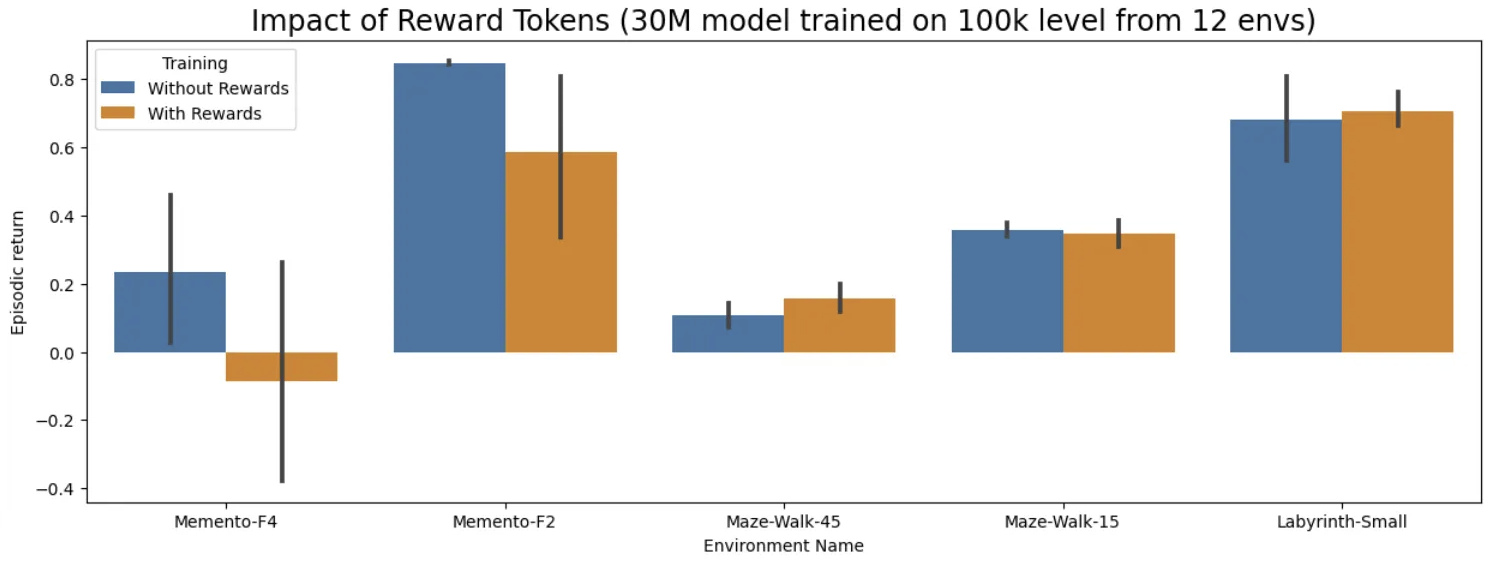
\includegraphics[width=0.7\columnwidth]{figures/reward_tokens.png}
    \caption{\textbf{Impact of Reward Tokens}: This figure illustrates the impact of reward tokens on the performance. Overall, reward tokens do not seem to play a crucial role in the performance across on all five MiniHack tasks. }
    \label{fig:reward_token}
\end{figure}

\subsection{Training Results}
In this section, we report the performance of our pre-trained models on the training environments.  We adhere to the same evaluation protocol specified in \Cref{sec:train_eval} and report the mean and standard deviation of the episodic return across three model seeds.
\subsubsection{MiniHack}
 We present the results in \Cref{fig:12_train}, \ref{fig:8_train}, and \ref{fig:4_train}. Overall, the performance is good on most of the environments and there is no big difference between the zero-shot and one-shot performance. This means that the model is utilizing the in-weights information to solve these tasks and conditioning on one-shot demonstration is not helping much. However, we notice that the model struggles to perform well on some tasks like /texttt{River Narrow, Corridor Battle} and \texttt{Lava Crossing}. We speculate that these environments are hard to solve and there is a high penalty for death. 


\begin{figure}[ht]
    \centering
    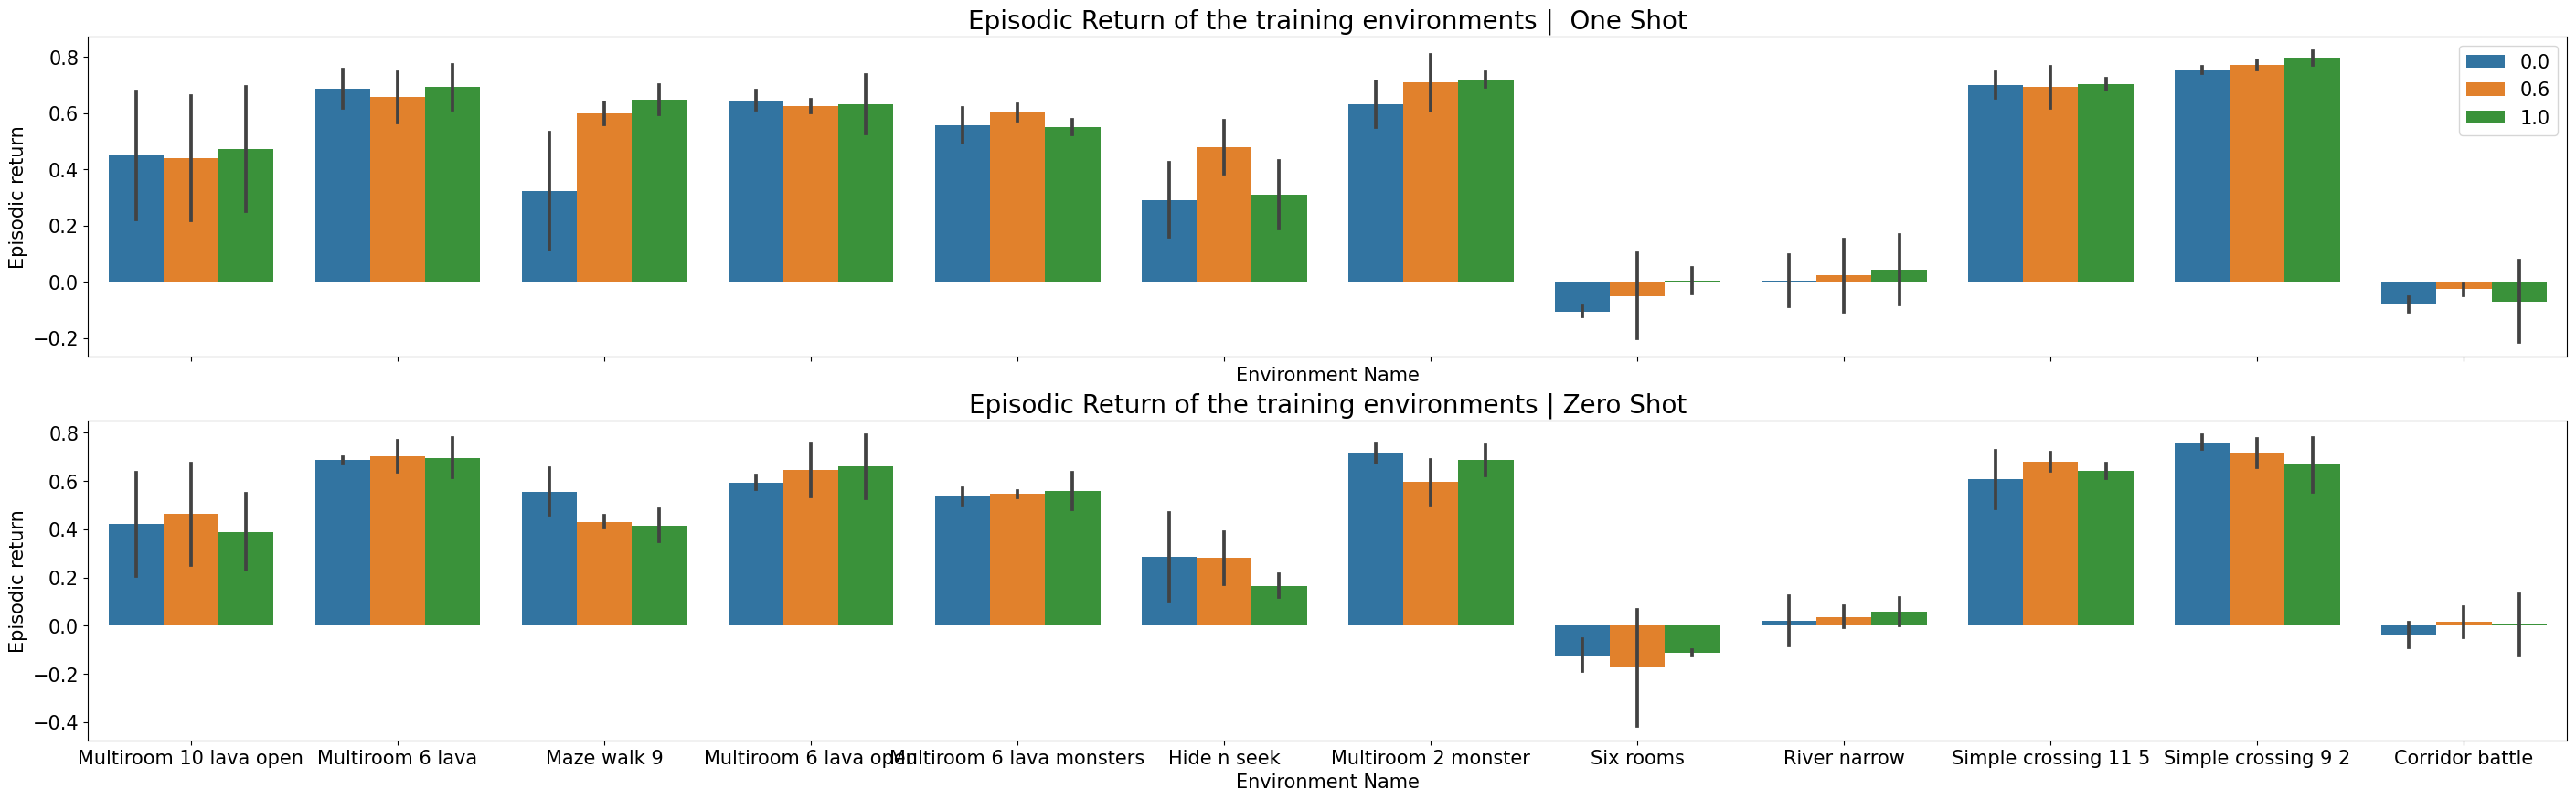
\includegraphics[width=0.8\columnwidth]{figures/12_envs_pretraining.png}
    \caption{\textbf{Performance on Test Levels from 12 Train Tasks} - This figure illustrates the episodic returns on 12 environments used for pre-training, across three different trajectory burstiness values; $p_b \in \{0.0, 0.6, 1.0\}$. Overall, the performance is good on most of the environments and there is no big difference between the zero-shot and one-shot performance. This means that the model is utilizing the in-weights information to solve these tasks, as expected. However, we notice that the agent's performance on \texttt{Corridor Battle, Six Rooms, River Narrow} is rather poor. }
    \label{fig:12_train}
\end{figure}


\begin{figure}[ht]
    \centering
    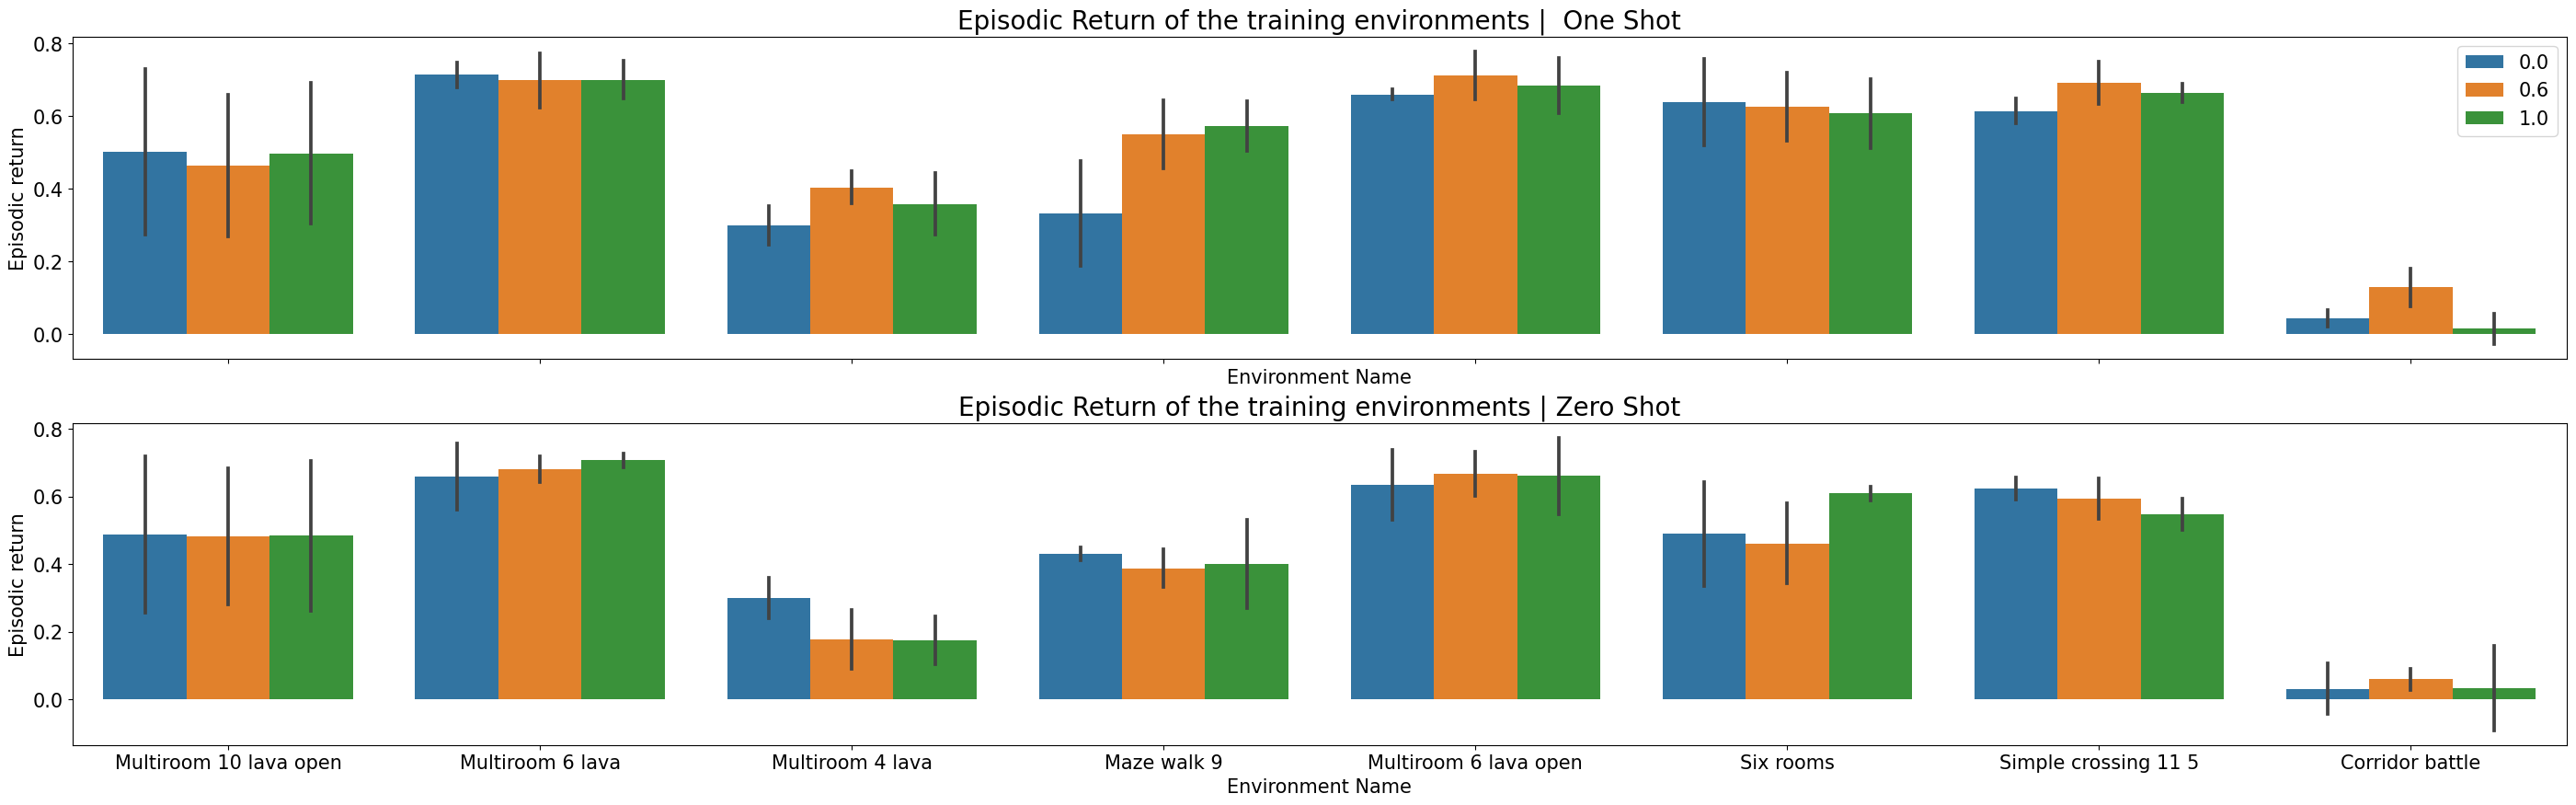
\includegraphics[width=0.8\columnwidth]{figures/8_envs_pretraining.png}
    \caption{\textbf{Performance on Test Levels from 8 Train Tasks} - This figure illustrates the episodic returns on 8 pretraining environments across three different trajectory burstiness values; $p_b \in \{0.0, 0.6, 1.0\}$. Overall, the performance is good on most of the environments and there is no big difference between the zero-shot and one-shot performance. This means that the model is utilizing the in-weights information to solve these tasks, as expected. However, we notice that the performance on \texttt{Corridor Battle} is rather poor. }
    \label{fig:8_train}
\end{figure}

\begin{figure}[ht]
    \centering
    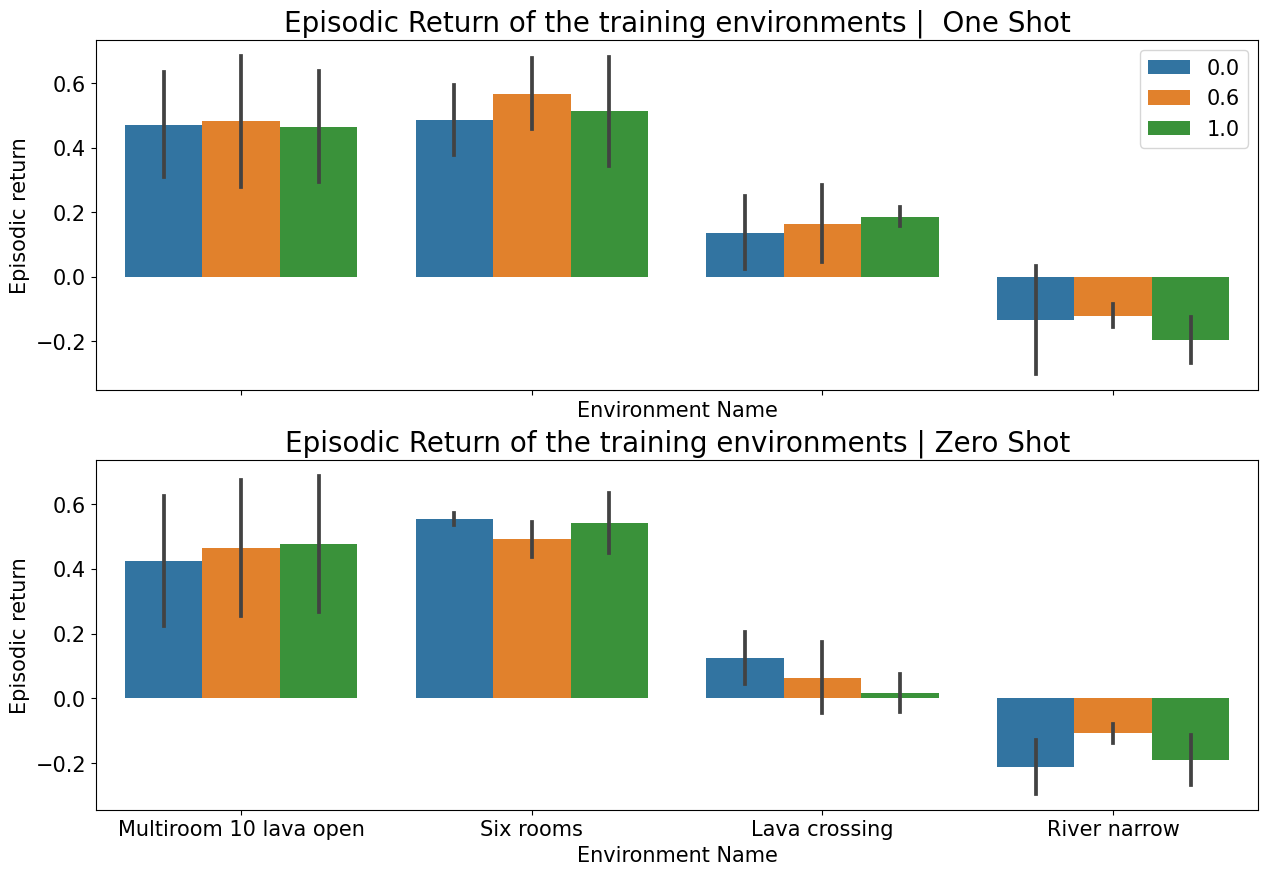
\includegraphics[width=0.5\columnwidth]{figures/4_envs_pretraining.png}
    \caption{\textbf{Performance on Test Levels from 4 Train Tasks} - This figure illustrates the episodic returns on 4 pretraining environments across three different trajectory burstiness values; $p_b \in \{0.0, 0.6, 1.0\}$. Overall, the performance is good on most of the environments and there is no big difference between the zero-shot and one-shot performance. This means that the model is utilizing the in-weights information to solve these tasks, as expected. However, we notice that the performance on \texttt{Lava Crossing, River Narrow} is rather poor.  }
    \label{fig:4_train}
\end{figure}
\subsubsection{Procgen} 
We present results in \Cref{fig:procgen_train}. We can see that the transformer model is able to perform consistently well across all the training environments. We also notice that there is not big difference in zero-shot and few-shot performance. 


\begin{figure}
    \centering
    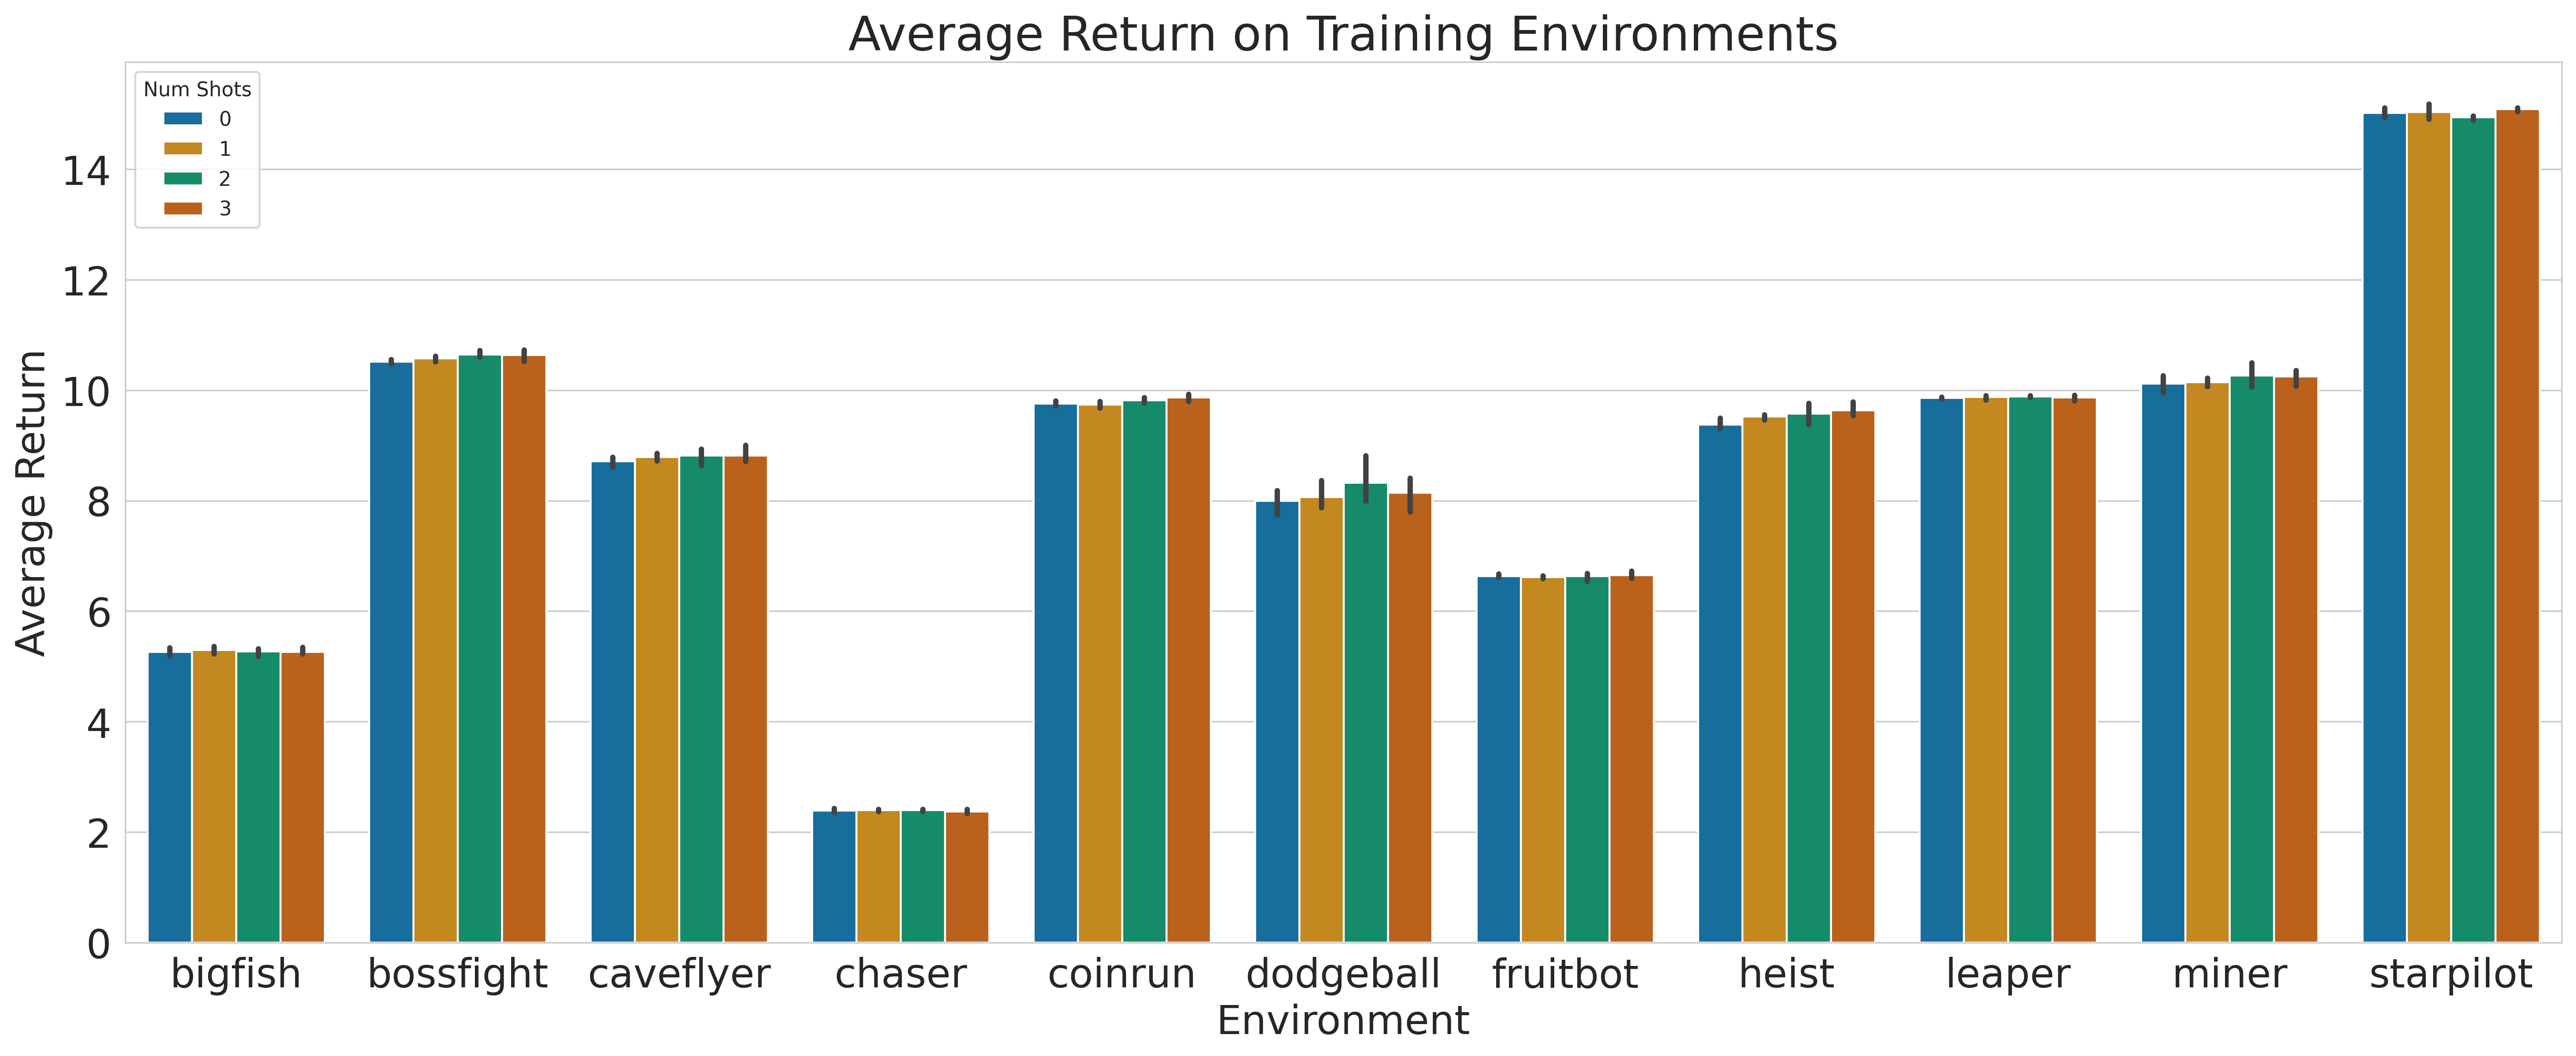
\includegraphics[width=\columnwidth]{figures/train_results.png}
    \caption{Procgen Train Environments Results. We observe that the model is able to perform well across all the training environments. }
    \label{fig:procgen_train}
\end{figure}
% \subsection{Burstiness Results}
\subsection{Task Diversity Results}
In this section, we extend the results presented in \Cref{sec:analysis} by showing the performance on unseen environments for a model pre-trained on 4 tasks. We can see that the claims made in  \Cref{sec:analysis} still hold - increasing the diversity of tasks improves generalization to new yet similar tasks via in-weights learning, but it is not clear how the diversity affects the model's ability to 'soft-copy' via in-context learning. In \Cref{app:env_scaling} we see that above a certain diversity of tasks, the in-context learning ability plateaus, while for lower task diversity, some novel tasks are capable of demonstrating in-context learning, while others are not.  
\begin{figure}[t]
    \centering
    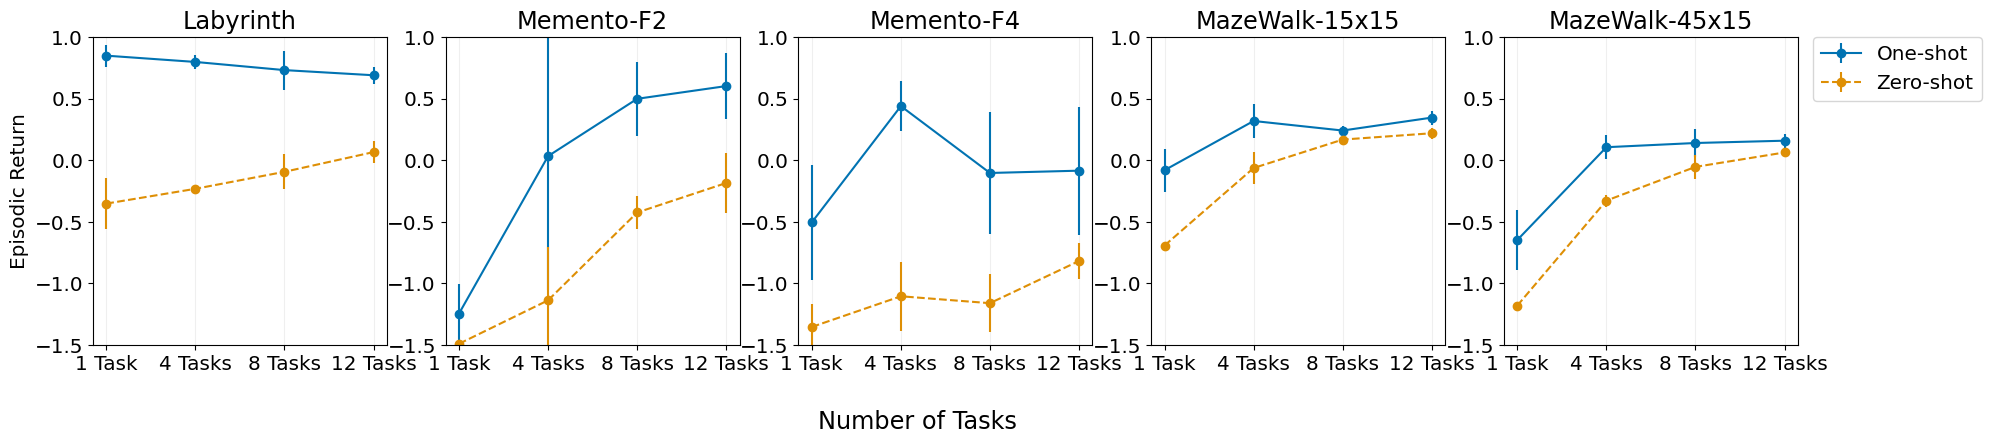
\includegraphics[width=\columnwidth]{figures/env_scaling_full.png}
    \caption{\textbf{Effect of Task Diversity}: This figure illustrates the effect of the number of different training tasks on the average episode return for 5 unseen MiniHack tasks. The dashed line indicates the zero-shot performance, and the solid line represents the one-shot performance. Overall, both the one-shot and zero-shot performances improve when increasing the number of tasks from 1 to 8, but then they plateau. This suggests that increasing the task diversity can help both the in-weights and in-context learning but the improvements have diminishing returns and may depend on the similarity between the train and test tasks. The error bars represent the standard deviation across 3 model seeds.}
    \label{app:env_scaling}
\end{figure}

% \subsection{Effect of Reward Tokens}
% In this section, we explore the importance of reward tokens for in-context learning. For all the experiments presented in the main paper, we process the sequences of the form $\{(s_0, a_0, r_0, s_1, a_1, r_1, \dots s_T, a_T, r_T)\}$ for each trajectory, where $s_i$ is the state, $a_i$ is the action and $r_i$ is the reward for the timestep $i \in 1, T$ . For the results presented in this section, we remove the reward information from the sequence and process the sequences of the form $\{(s_0, a_0, s_1, a_1, \dots s_T, a_T)\}$. 

% \section{Limitations}
% In this section, we will discuss the limitations of our work. One of the limitations of our study, as noted in \Cref{sec:env_difficulty}, is the model's sensitivity to covariate shifts and  unforgivemness of the environments. The few-shot experiments presented in \Cref{sec:main_expts} do offer some mitigation to these concerns, we believe that there is still a lot of room for investigation here. Furthermore, since our study is heavily on expert demonstrations, our model's efficacy might be limited when presented with non-expert demonstrations. Addressing these areas could offer valuable directions for future research endeavors.
% We hypothesize that increasing the context length and presenting the model with few-shot demonstrations, as opposed to a single demonstration, should improve performance on the tasks like \texttt{Memento-F4}, \texttt{River Narrow} and \texttt{Lava Crossing}. Another limitation of our work is that all the results are based only on MiniHack environments. While the results are promising, it is not clear if the results are valid on other benchmarks. As a future work, we would like to study the applicability of the claims made in the paper on existing popular benchmarks like Procgen ~\cite{cobbe2020leveraging}. 

\subsection{Procgen Sticky Action Results}
\label{app:procgen_sticky}
In this section, we perform evaluations on Procgen test environments with sticky actions with sticky probability 0.3 (higher than what we consider in \Cref{sec:main_expts}). We follow similar evaluation protocol as mentioned in \Cref{sec:main_expts} and report the performance across 5 procgen tasks. As we can see, the performance of our model is consistent with the performance in \Cref{fig:Procgen_results_sticky}. While we outperform the most of the baselines, the Hashmap is competitive in case of plunder. Despite the increase in stochasticity, we find our main conclusions are inline with \Cref{sec:main_expts}.

\begin{figure}
    \centering
    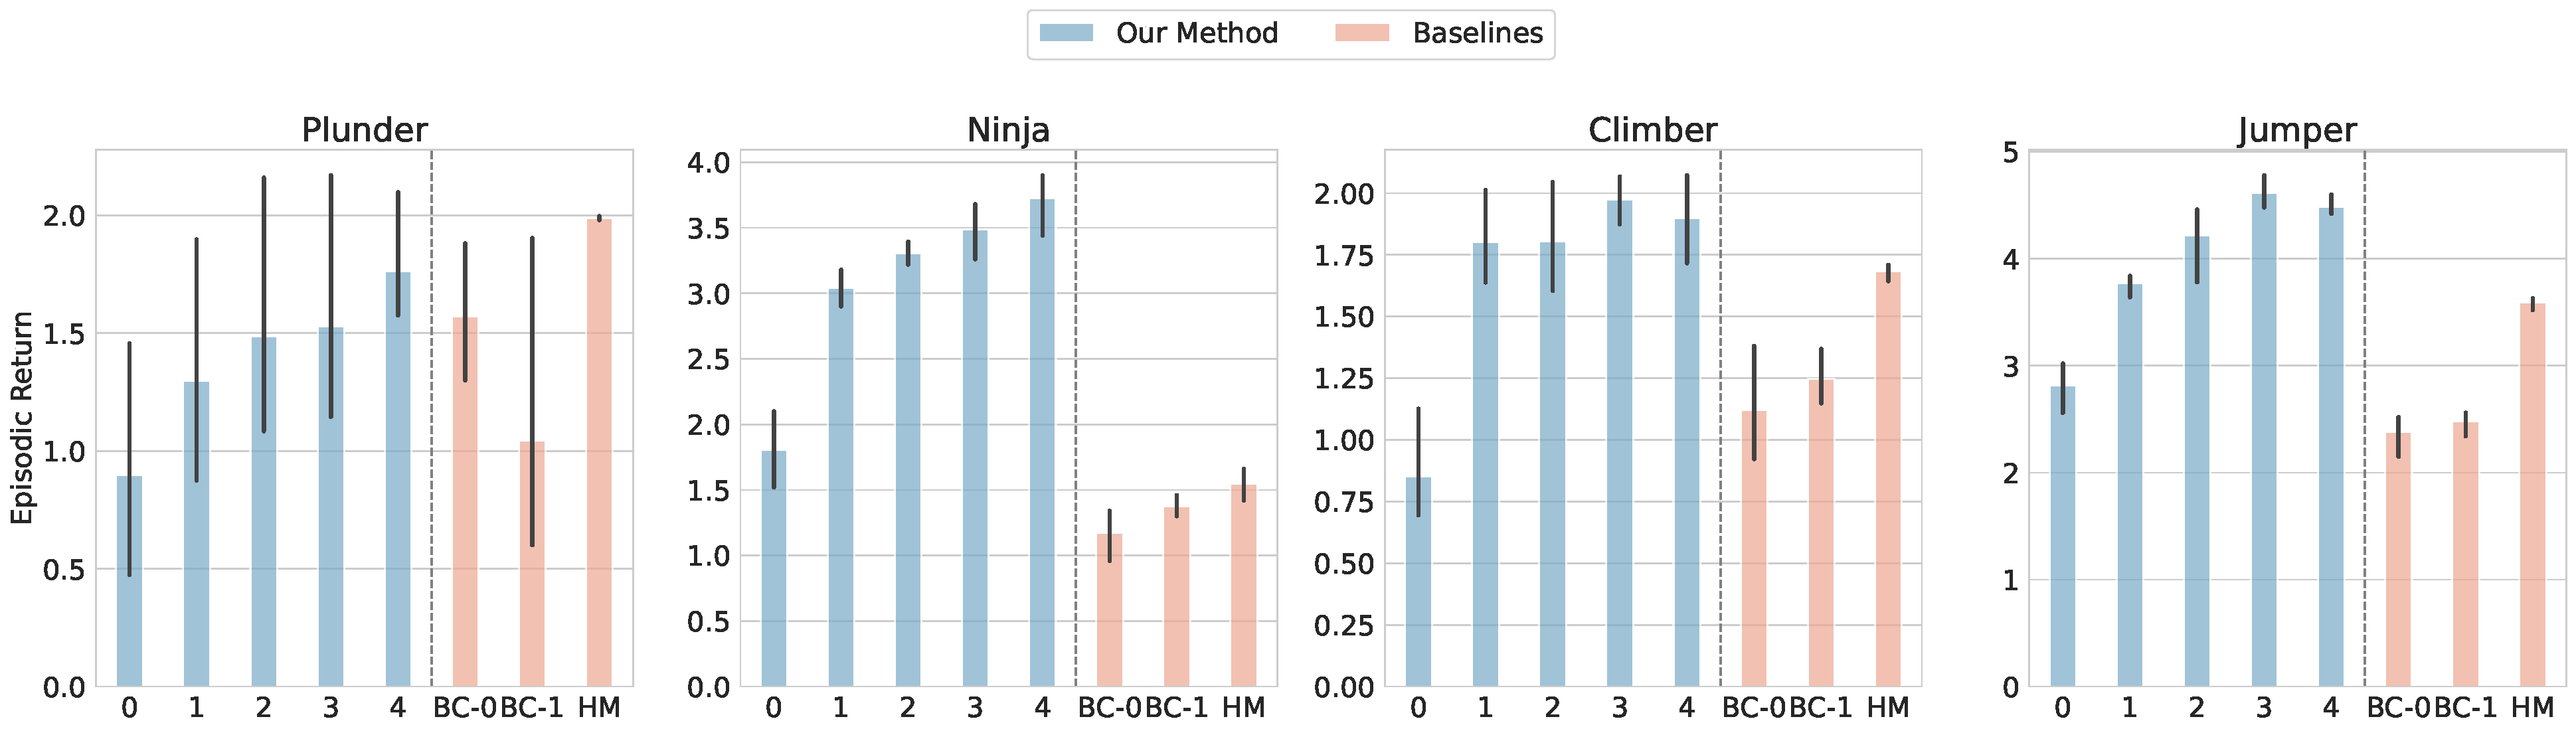
\includegraphics[width=0.8\columnwidth]{figures/few_shot_results_procgen_1_train_0.3.pdf}
    \caption{\textbf{Sticky Action Evaluations} comparing (1) our multi-trajectory transformer conditioned on different number of demonstrations from the same level, (2) Hashmap baseline conditioned on the same demonstrations, and (3) BC baseline conditioned on zero and one demonstration due to context length constraints. 
    % Our model outperforms both baselines when provided with at least one demonstration and its performance improves with the number of demonstration. 
    }
    \label{fig:Procgen_results_sticky}
\end{figure}
% \subsection{Effect of Training Distribution in ProcGen}
% In this section, we conduct experiments to understand how varying the mix of tasks during training influences performance on downstream tasks. Our observations, as depicted in \Cref{procgen_training_splits}, indicate that the distribution of training tasks does have an impact on certain downstream tasks. However, we posit that the significance of this effect reduces when the training is conducted at a larger scale.
% \begin{figure}[ht]
%     \centering
%     \begin{subfigure}[b]{0.8\columnwidth}
%         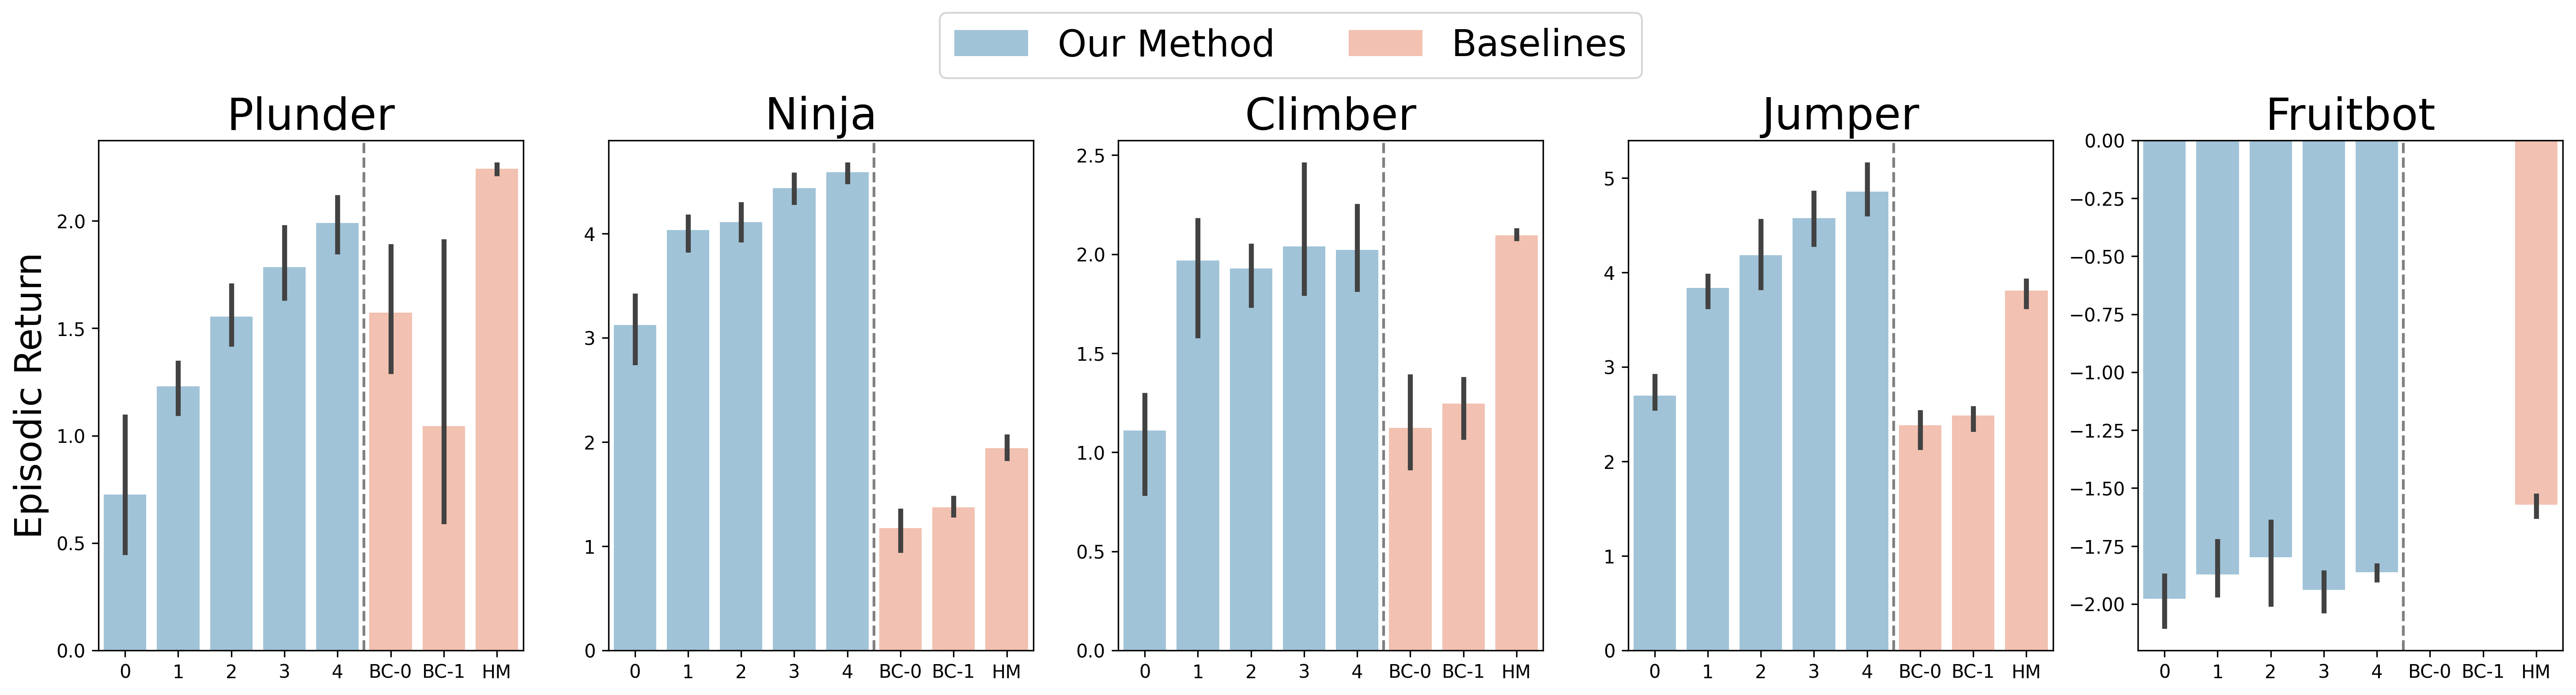
\includegraphics[width=\textwidth]{figures/few_shot_results_procgen_new_dit_1.png}
%         \caption{Training split 1}
%         \label{fig:Procgen_results_1}
%     \end{subfigure}
%     \hfill % Optional: add some space between the two subfigures
%     \begin{subfigure}[b]{0.8\columnwidth}
%         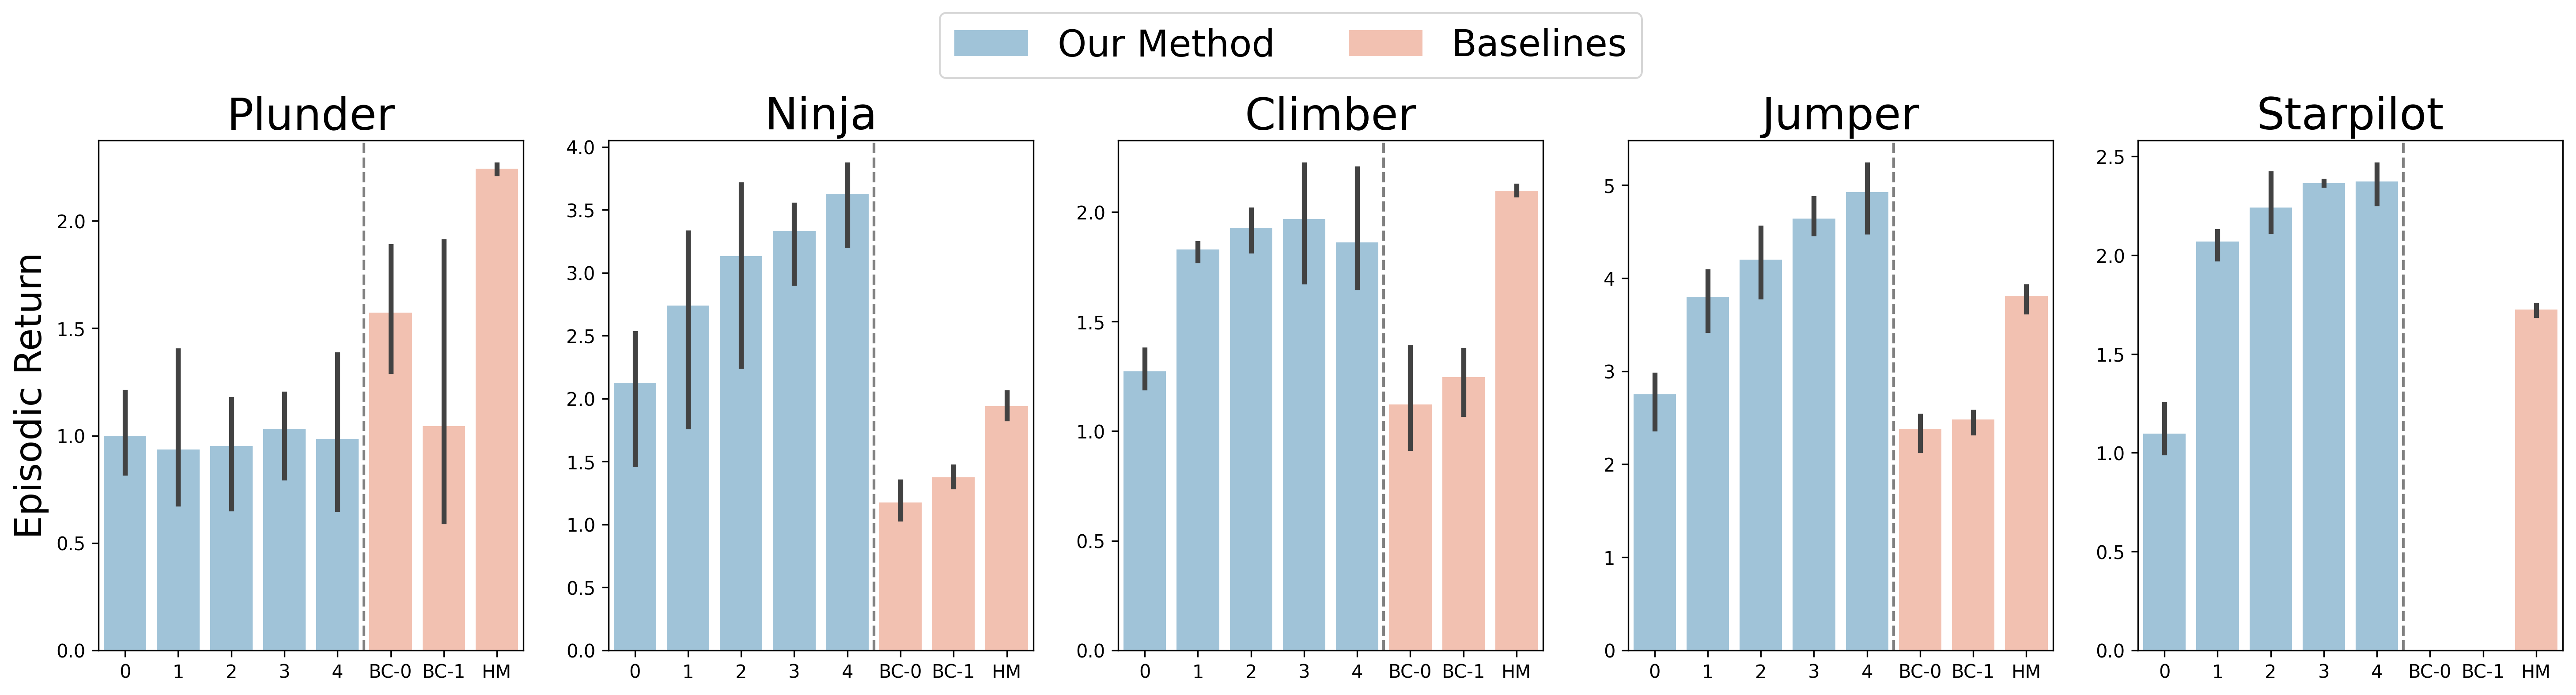
\includegraphics[width=\textwidth]{figures/few_shot_results_procgen_new_dit_2.png}
%         \caption{Training split 2}
%         \label{fig:Procgen_results_2}
%     \end{subfigure}
%     \caption{Comparisons of our multi-trajectory transformer with baselines on ProcGen tasks with different training splits. }
%     \label{fig:procgen_training_splits}
% \end{figure}



\section{Broader Impact}

The ability to generalize to unseen tasks with the help of single demonstration is crucial for many real world applications like robotics, self-driving cars. In this work we focus on how to achieve this goal with the help of in-context learning. More specifically, our work focuses on highlighting how different factors like trajectory burstiness $p_b$, environment dynamics, task dynamics, model and dataset sizes influence in-context learning in sequential decision-making settings. Since our results are based on Minihack and Procgen environments, which are somewhat simplified comapared to real-world settings, we do not foresee any potential negative impact on the society. We believe that our work could provide some useful insights into using transformers for sequential decision-making settings. 

\section{Hyperparameters}
We present the hyperparameters used in this work in \Cref{tab:hps}
\begin{table}[h]
    \centering
    \begin{tabular}{c c}
        \hline
\textbf{Hyperparameters} & \textbf{Values} \\
\hline
Batch Size & 64 \\
Number of Levels & \{ 10000, 30000, 100000\} \\
Context Size & 900 \\
Vocabulary Size & 32 \\
Trajectory Burstiness $p_b$ & \{ 0.0, 0.6, 1.0 \} \\
Sticky Probability & 0.2 \\
Number of Epochs & 25 \\
Learning Rate & 0.0001 \\
Learning Rate Scheduler & Consine Annealing \\
Minimum Learning Rate & 1.0e-06 \\
Model Size & \{128, 256, 512, 768, 1024 \} \\
Number of Layers & \{ 4, 6, 8, 12,\} \\
Number of Heads & \{ 4, 8, 12 \} \\
Vocabulary Size & 32 \\
Dropout & 0.2 \\
Nethack Hidden Size & 64 \\
Nethack Embedding Size & \{128, 256, 512, 768 \} \\
Crop Size & 12 \\
Nethack Number of Layers & 2 \\
Nethack Dropout & 0.1 \\
\hline
    \end{tabular}
    \caption{List of hyperparameters used in our experiments}
    \label{tab:hps}
\end{table}
